\section{讨论}该节用于对研究结果进行讨论,讨论的基础是结果与分析,应在对结果透彻理解的基础上归纳研究的主要结果,从中得
出的主要结论,阐述与前人的研究结果相比有什么进步,解决了什么科学问题,研究结果在理论上和应用上的价值、前景等(\textbf{在本模板中,这节用来展示表格,伪代码,代码块与图片的插入})

\subsection{表格}
\par 本来LaTeX里表格的变化是非常多的,在规范要求中,学校统一要求使用3线表。以下是一个3线表的例子(该方法可以较好的平均分配\textbf{与文档同宽的表格}的列间距,同时保证每一列是居中排列):

\begin{table}[htbp] 
	\centering
	
	% 中文表题开始
	\caption{示例表格}
	% 中文表题结束
	
	% 英文表题开始
	\addtocounter{table}{-1}
	\vspace{-5pt}
	\renewcommand{\tablename}{Table}
	\caption{Example Table}
	% 英文表题结束
	
	\begin{spacing}{1.5}
		\begin{tabular*}{\textwidth}{@{\extracolsep{\fill}} cccc}
			\toprule
			栏目一 & 栏目二 & 栏目三 & 栏目四 \\
			\midrule
			内容1 & 内容2 & 内容3 & 内容4 \\
			内容5 & 内容6 & 内容7 & 内容8 \\
			内容9 & 内容10 & 内容11 & 内容12 \\
			内容13 & 内容14 & 内容15 & 内容16 \\
			内容17 & 内容18 & 内容19 & 内容20 \\
			% 可以添加更多的行
			\bottomrule
		\end{tabular*}
	\end{spacing}
\end{table}

\par 图表将以表 1(Table 1)、表 2(Table 2 ),图 1(Fig. 1)、图 2(Fig. 2)等统一编号。每个图表都应有标题,内容应简单明了,中英文对照,居中排列。表题置于表的上部,图题置于图的下方。(加入对照的中英文表题/图题的步骤,可参考\url{http://t.csdnimg.cn/zYHw7})

\subsection{伪代码}
\par 如果你的论文中出现需要用到伪代码来描述的算法流程,可以参考如下表格(以迪杰斯特拉算法为例):

\setlength{\intextsep}{10pt plus 2pt minus 2pt} % 调整上下间距
\begin{table}[t] % 此处为了美观将伪代码表格置顶了,在使用过程中请根据自身需要调整
	\centering
	\caption{Dijkstra 算法伪代码}
	\begin{spacing}{1.25}
	\begin{tabular*}{\textwidth}{@{\extracolsep{\fill}} p{\textwidth}}
		\toprule
		\textbf{Dijkstra 算法} \\
		\midrule
		\begin{algorithmic}[1]
			\Procedure{Dijkstra}{$G, s$}
			\State 初始化距离数组 $d$ 至所有节点为 $\infty$
			\State 设置起始点 $s$ 的距离 $d[s] = 0$
			\State 初始化未访问节点集合 $Q$
			\While{$Q$ 不为空}
			\State 从 $Q$ 中取出距离最小的节点 $u$
			\State 从 $Q$ 中移除节点 $u$
			\For{每一个邻接点 $v$ 于 $u$}
			\State $alt \gets d[u] + \text{length}(u, v)$
			\If{$alt < d[v]$}
			\State 更新距离 $d[v] \gets alt$
			\EndIf
			\EndFor
			\EndWhile
			\State \textbf{return} $d$
			\EndProcedure
		\end{algorithmic} \\
		\bottomrule
	\end{tabular*}
\end{spacing}
\end{table}
\setlength{\textfloatsep}{10pt plus 2pt minus 2pt} % 调整上下间距

\subsection{代码块}
\par 如果你的论文中出现需要展示处理分析数据用到的源代码(通常放在附录中),还是以迪杰斯特拉算法为例,可参考如下代码块:
\begin{lstlisting}[caption={Dijkstra 算法的 Python 实现}, label={lst:dijkstra}]
	import heapq
	
	def dijkstra(graph, start):
	distances = {vertex: float('infinity') for vertex in graph}
	distances[start] = 0
	queue = [(0, start)]
	
	while queue:
	current_distance, current_vertex = heapq.heappop(queue)
	
	if current_distance > distances[current_vertex]:
	continue
	
	for neighbor, weight in graph[current_vertex].items():
	distance = current_distance + weight
	
	if distance < distances[neighbor]:
	distances[neighbor] = distance
	heapq.heappush(queue, (distance, neighbor))
	
	return distances
\end{lstlisting}


\subsection{插图}
\par 由于这份模板不考虑多栏排版,所以以下是通栏图的演示:
\begin{figure}[H]
    \centering
    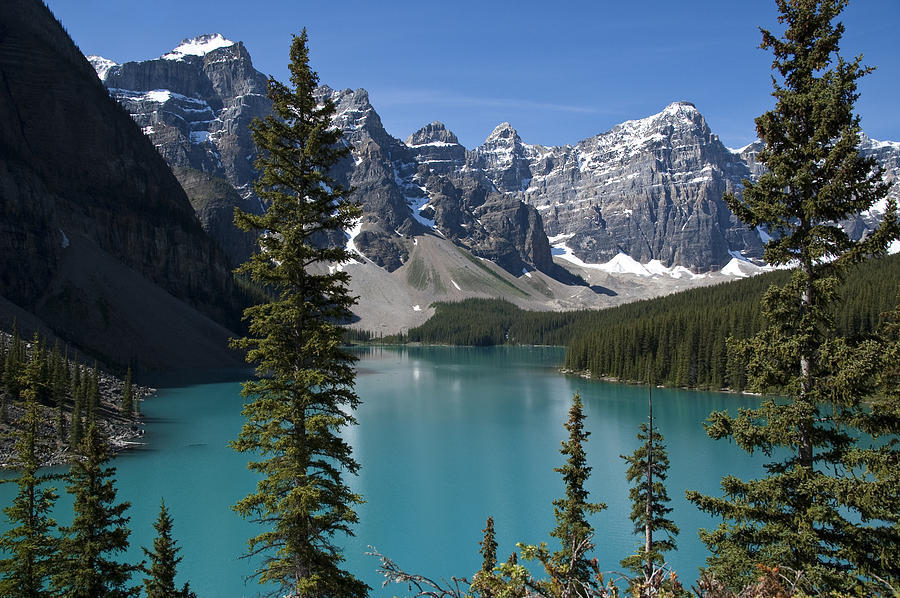
\includegraphics[width=100mm]{./figures/Example.jpg}
    \caption{图片测试} 
    
    % 英文表题开始
    \addtocounter{figure}{-1}
    \vspace{-5pt}
    \renewcommand{\figurename}{Figure}
    \caption{Image test}
    % 英文表题结束
    
\end{figure}


\par 当你需要将两个相同大小的图片排列在同一行时(例如需要比较两张图片中的曲线变化时),可参考以下环境:
\begin{figure}
	\centering
	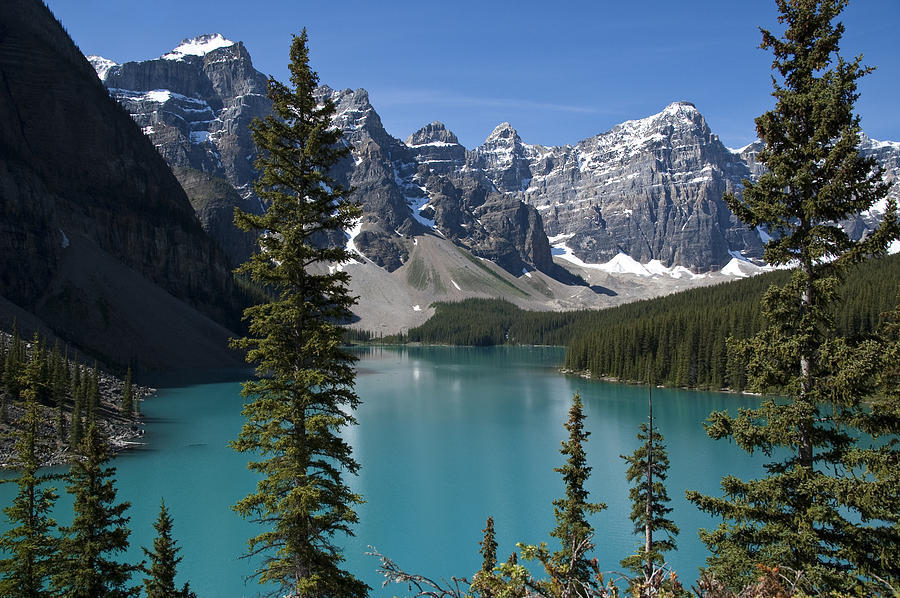
\includegraphics[scale=0.5]{./figures/Example.jpg}
	\hspace{1in}
	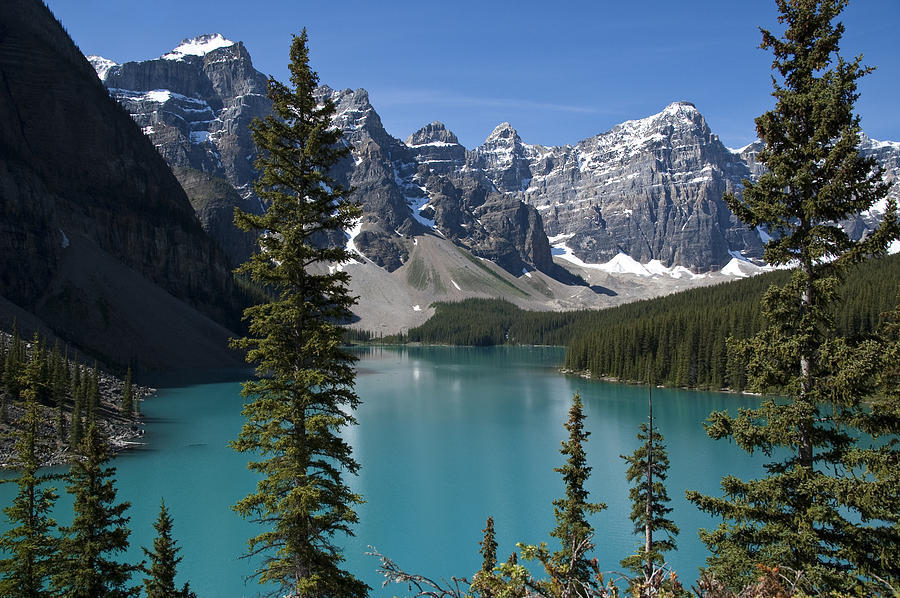
\includegraphics[scale=0.5]{./figures/Example.jpg}
	\caption{两张图片并排在一个浮动体}
	
	% 英文表题开始
	\addtocounter{figure}{-1}
	\vspace{-5pt}
	\renewcommand{\figurename}{Figure}
	\caption{Two images placed side by side in a floating body}
	% 英文表题结束
\end{figure}
\par 这是两张图片共享一个图题的模板,若两张图的图题不相同,参考如下:

\begin{figure}
	\begin{minipage}[t]{0.5\linewidth}
		\centering
		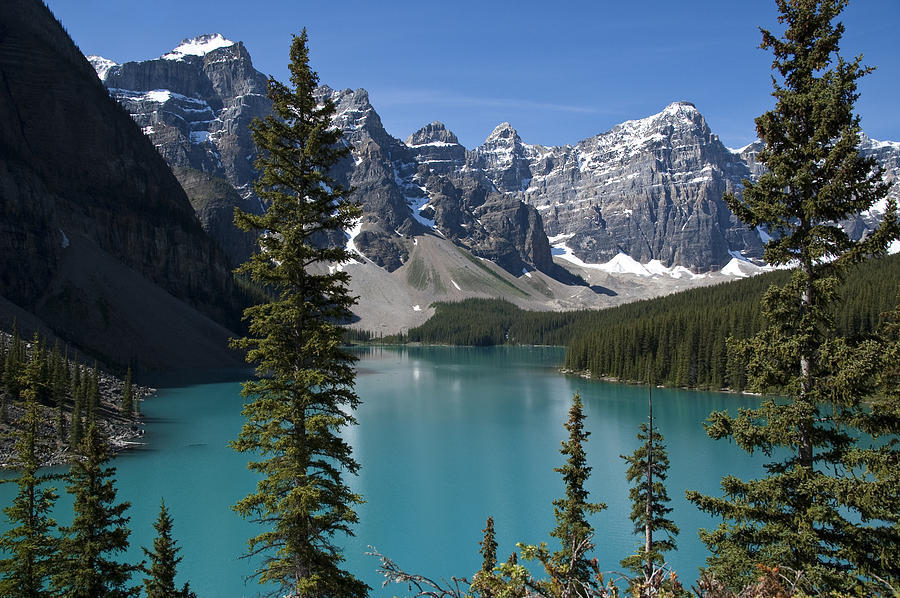
\includegraphics[scale=0.5]{./figures/Example.jpg}
		\caption{ABCD}
		
		% 英文表题开始
		\addtocounter{figure}{-1}
		\vspace{-5pt}
		\renewcommand{\figurename}{Figure}
		\caption{ABCD}
		% 英文表题结束
		
		\label{fig:side:a}
	\end{minipage}%
	\begin{minipage}[t]{0.5\linewidth}
		\centering
		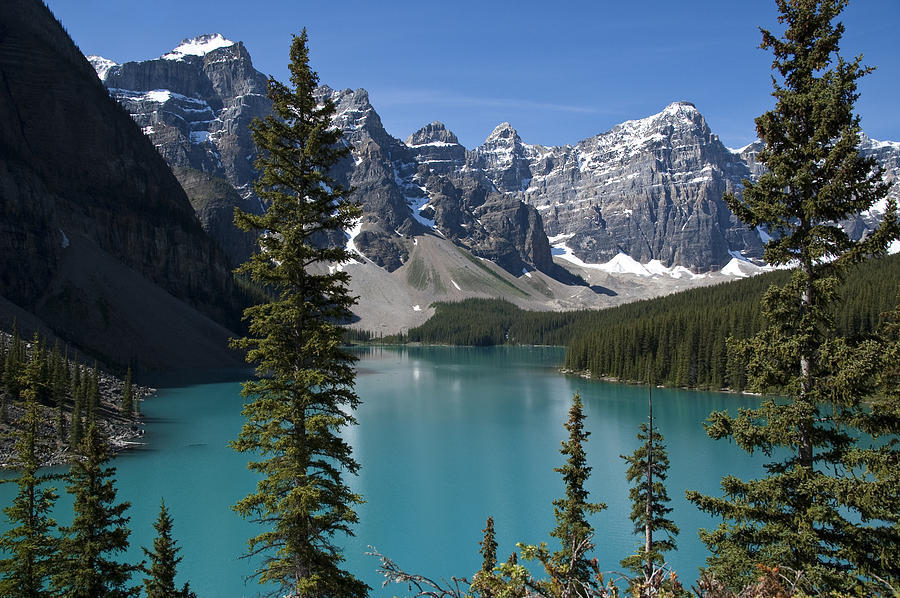
\includegraphics[scale=0.5]{./figures/Example.jpg}
		\caption{abcd}
		
		% 英文表题开始
		\addtocounter{figure}{-1}
		\vspace{-5pt}
		\renewcommand{\figurename}{Figure}
		\caption{abcd}
		% 英文表题结束
		
		\label{fig:side:b}
	\end{minipage}
\end{figure}

\par 注意:这里为了减少图片上下的空白,使用了float宏包。